 \documentclass[12pt,a4paper,twoside]{book}
\usepackage[utf8]{inputenc}
\usepackage[english]{babel}
\usepackage{preamble}
\setcounter{secnumdepth}{3}
\setcounter{tocdepth}{3}
%The bibliography is made with BibLaTeX, not BibTeX. To compile with BibLaTeX, substitute "bibtex %.aux" with "biber %" in the Bib(la)tex voice you can find in TexMaker configuration menu.
\usepackage[backend=biber,style=chem-acs]{biblatex}
\addbibresource{biblio.bib}

\begin{document}
%TITLEPAGE-----------------------------------------------------
\thispagestyle{empty}
\begin{center} 
\includegraphics[scale=.28]{logo}
\vspace{.5 cm} \\
{\LARGE \sc \color{reddy} University of Pavia}
\vspace{1 cm} \\
{\Large \sc Master's Degree Thesis} \vspace{1 cm}\\
\hrule height 1 pt \vspace{1cm}
\LARGE  Dr. Bianchi's Thesis Template Explained \\ \normalsize \it -- directly on his template --
\vspace{1cm}
\hrule height 1 pt
\end{center}
\vspace{1 cm}
\begin{center}
\begin{minipage}{.9\textwidth}
{\it Author: \hfill Supervisor:} \\
{\color{reddy} Alessio Bianchi \hfill Your Supervisor's name} \\ \\
\phantom{x} \hfill \textit{Co-Supervisor:}\\
\phantom{x} \hfill {\color{reddy} Your Co-Supervisor's name} \\
\end{minipage}
\vfill
{\it A thesis submitted in fullfillment of the requirements for the} \\ \ \\
{\color{reddy} Master's Degree in Chemistry} \\ \ \\
{\it in the} \\ \ \\
{\color{reddy} Department of Chemistry \\ Organic Chemistry Section}
\\ \ \\
July, 2022
\end{center}
\newpage
\thispagestyle{empty}

\begin{flushright}
\begin{minipage}{.9\textwidth}
{\bf \LARGE\hfill\color{reddy}  Abstract} \vspace{20 pt}\\
%\addcontentsline{toc}{chapter}{Abstract}
Give thanks to the mother Gaia, give thanks to the father sun; give thanks to the plants in the garden where the mother and father are one.
\end{minipage}
\end{flushright}

%TOC------------------------------------------------------------
\small
\frontmatter %uses roman pagenumbers
\dominitoc
\setstretch{1.2}
{\small  \tableofcontents}
\newpage
\thispagestyle{plain}
%BODY---------------------------------------------------
\normalsize
	\mainmatter %the body of your thesis with arabic page numbers
	\setstretch{1}
%	\part{Using Parts is Not Mandatory, Actually}

	\chapter{Introduction}
	
\section{Background}

\section{Research aims and motivation}

\section{Objectives and scope}

\section{Thesis statement and hypothesis}

\section{Overview and structure of thesis}

	\chapter{Literature Review}
	
\section{Overview}

\section{Methodologies for analysing the effect of land cover change}

\subsection{Approaches}

\subsection{Datasets and models}

\section{Findings and results on the effect of land cover change on surface winds}

\subsection{Observed changes in near-surface wind speed over the last few decades}

\subsubsection{Slowdown and "global terrestrial stilling"}

\subsubsection{Trend reversal and large-scale ocean-atmosphere circulations}

\subsubsection{Instrument drift}

\subsection{Conversion of agricultural land into urban centres}

\subsubsection{Rate of urbanisation and size of cities}

\subsubsection{Urban heating effects}

\subsubsection{Anomalies and the "urban wind island effect"}

\subsection{Conversion of natural forest into agricultural land}

\subsubsection{Roughness length changes}

\subsubsection{Teleconnections}

\section{Vegetation-atmosphere interactions and their possible mechanisms}

\subsection{Secondary organic aerosols}

\subsection{Convective cloud development}

\subsection{Surface and latent heat fluxes}

\subsection{Surface temperature and pressure}

	\chapter{Methodology}

\section{Approach}

\subsection{Focus regions}

\subsubsection{Central America}

\subsubsection{South America}

\subsubsection{Western Australia}

\subsection{Statistical metrics}

\subsubsection{Mean diurnal profile climatology}

\subsubsection{Weibull parameters}

\section{Reproducibility}

\section{Datasets}

\subsection{Reanalysis data for atmospheric variables}

\subsection{Long-term satellite-derived products for land surface variables}

\section{Software}

	\chapter{Results}
	
\section{Central America}

\section{South America}

\section{Western Australia}

	\chapter{Discussion}
	
\section{Interpretation of results}

\section{Comparison with literature}

\section{Significance}

\section{Limitations and possible improvements}

\section{Future directions for research}

	\chapter{Conclusions}
	
\appendix

	\chapter{Supplementary information and graphs}
	
\section{Comparison of leaf area index datasets}
	
	\chapter{Data, files and codebooks}
	
\section{Availability and reproducible results}
	
\section{Description of analysis functions}

	\chapter*{Probably, The Introduction} 
	\epigraph{\it A cool citation is always an extra-point.}{-- Someone Important}
	\minitoc
		\setstretch{1.2}
\section*{A Little Overview}
This template has been directly made by modifying the common \LaTeX 's {\color{reddy} \verb|book|} documentclass. You can find the related code, with comments, in the {\color{reddy} \verb|preamble.sty|} file. The default font-family is {\color{reddy} \verb|Liunx Libertine/Biolinum|} in which the second one -- Sans variant -- is set as default, while math environments like this
$$x(t)=A\sin(\omega t + \phi)$$
use the Serif variant: nobody forbids you from using different fonts (like the ones already included in the preamble or completely different).
\subsection*{The Color Accent}
The document possesses a color accent called ‘{\color{reddy} \verb|reddy|}’ which is used for chapter titles, footnotes numbers,\footnote{Like this one.} bullets in lists, and others. You can recall it to color-up your stuff with {\color{reddy} \verb|\color{reddy}|} and modifying its RGB color definition in the preamble file also.

\subsection*{The \texttt{preamble.sty} File}
The preamble file contains adjustments in margins, tables, headers and footers, and a lot of other stuff: the best piece of advice I can give you is... {\color{reddy} go check-it-out}! Don't worry: it is all commented. The print format is on twosided pages, but it can be set as oneside -- but remember to correct headers and footers code lines!

\section*{Setting the Bibliography}
For references management, I \underline{\color{reddy} \bf hardly} recommend the usage of {\color{reddy} Bib\LaTeX}  instead of the more common Bib\TeX . In fact, {\color{reddy} Bib\LaTeX} has got a lot less bugs and it is more easy and intuitive to compile. Furthermore, it only needs the classical \verb|.bib| file in your working directory and it is also able to cite something directly as a footnote like this.\footfullcite{Wang2021} Notice that the citation is also reported in the bibliography section and that the default citation style set is \textit{American Chemical Society}, but you can obviously change it, according to your needs, at the very beginning of this {\color{reddy} \verb|Thesis.tex|} document code.

\subsection*{Automatically Compile Bib\LaTeX \ through \tt biber}
Many \LaTeX \ editors do not have a specific shortcut for {\color{reddy} \verb|biber|}, the main Bib\LaTeX\ compiler. You can manually add a shortcut with the command
\begin{verbatim}
biber %
\end{verbatim}
 or, if you use \TeX Maker like me, you can go to {\color{reddy} \texttt{Options $\to$ Configure Texmaker $\to$ Commands}} and put it in the \verb|Bib(la)tex| box instead of \verb|bibtex %.aux| ({\color{reddy}\bf Figure \ref{window}}).

\begin{figure}[h]
\centering
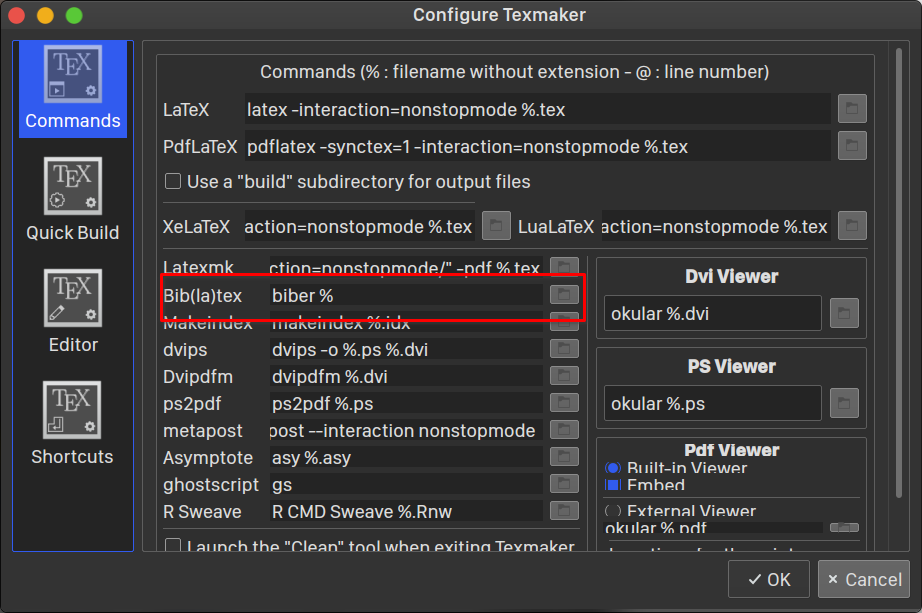
\includegraphics[width=.7\textwidth]{biber}
\caption{\TeX Maker's dialogue window to change Bib(la)tex command for compiling a Bib\LaTeX\ bibliography.}
\label{window}
\end{figure}

\section*{Credits}
This template was made by Dr. Alessio Bianchi (University of Pavia, Department of Chemistry, Organic Chemistry Section). For support, please contact me \href{mailto:alessio.bianchi02@universitadipavia.it}{\bf \color{reddy}$\to$ via mail~$\leftarrow$} and go check-out my homepage at \href{https://bianchiunipv.wordpress.com/}{\color{reddy} bianchiunipv.wordpress.com} to find other interesting stuff.\newline \\
I hope this will be useful and comfortable in usage! And... break a leg for you degree ;)

	\setstretch{1}
	\chapter*{Empty Chapter} 
	\epigraph{\it A cool citation is always an extra-point.}{-- Someone Important}
	\minitoc
		\setstretch{1.2}
\section*{Hint}
Just copy-paste this block for new chapters.

\backmatter % the format for the end of your thesis
%\part{End Sections}
\pagestyle{plain}
\begin{footnotesize}
\addcontentsline{toc}{chapter}{Bibliography}
%{\LARGE \bf \hfill \color{reddy} Bibliography}% <- TO BE REMOVED WHEN BIBLIOGRAPHY IS LOADED
%\bibliographystyle{acs} %<--- Uncomment if you wanna use BibTex Instead of BibLaTeX
%\bibliography{biblio.bib} %<--- Uncomment if you wanna use BibTex Instead of BibLaTeX
\printbibliography
\end{footnotesize}
\newpage
%\addcontentsline{toc}{chapter}{Appendix}
%{\LARGE \bf \hfill \color{reddy}Appendix}
%\newpage
\listoffigures
\addcontentsline{toc}{chapter}{List of Figures}
\listoftables
\addcontentsline{toc}{chapter}{List of Tables}
\newpage
\vspace*{1.5cm}
\begin{flushright}
\begin{minipage}{.9\textwidth}
{\bf \LARGE\hfill\color{reddy}  Acknowledgements} \vspace{20 pt}\\
\addcontentsline{toc}{chapter}{Acknowledgements}
Give thanks to the mother Gaia, give thanks to the father sun; give thanks to the plants in the garden where the mother and father are one.
\end{minipage}
\end{flushright}
\end{document}

